\documentclass[bigchapter,type=bsc,colorback,accentcolor=tud11b]{tudthesis}

%--------------------------------------------------------
% shows reference keys
%--------------------------------------------------------
%TODO: remove for final
%\usepackage{showkeys}

%--------------------------------------------------------
% provides the todo command
%--------------------------------------------------------
\newcommand\todob[1]{{\color{red}\fbox{
\begin{minipage}{\textwidth-4pt}\texttt{ TODO: #1 }\end{minipage}}}}

\newcommand\todo[1]{{\color{red}\fbox{\texttt{\footnotesize TODO: #1}}}}

%--------------------------------------------------------
% more package references
%--------------------------------------------------------
%\usepackage{ngerman}   ...ist ja gar nicht auf deutsch!
\usepackage{booktabs}
\usepackage{tabularx}

\usepackage{hyperref}

\usepackage{varwidth}

\usepackage{graphicx}
\usepackage{wrapfig}

\usepackage[bibencoding=utf8]{biblatex}
%\usepackage{parskip}

% new page for each section
%\usepackage{titlesec}
%\newcommand{\sectionbreak}{\clearpage}

% flow charts etc.
\usepackage{tikz}
\usetikzlibrary{shapes,arrows,positioning,automata}

\usepackage{listings}

%--------------------------------------------------------
% configuration
%--------------------------------------------------------

%\bibliographystyle{IEEEtran}
\bibliography{thesis-h2-mptcp}

\setlength{\parskip}{0.75\baselineskip}%
%\setlength{\parindent}{0pt}%

% increase line height
\renewcommand{\baselinestretch}{1.2} 

\newcommand\code[1]{\texttt{\detokenize{#1}}}

% german month for TUDthesis
\newcommand{\getmydate}{%
	\ifcase\month%
	\or Januar\or Februar\or M\"arz%
	\or April\or Mai\or Juni\or Juli%
	\or August\or September\or Oktober%
	\or November\or Dezember%
	\fi\ \number\year%
}

\definecolor{mygreen}{rgb}{0,0.6,0}
\definecolor{mygray}{rgb}{0.5,0.5,0.5}
\definecolor{mymauve}{rgb}{0.58,0,0.82}

\lstset{ %
  basicstyle=\footnotesize,        % the size of the fonts that are used for the code
  breakatwhitespace=false,         % sets if automatic breaks should only happen at whitespace
  breaklines=true,                 % sets automatic line breaking
  captionpos=b,                    % sets the caption-position to bottom
  commentstyle=\color{mygreen},    % comment style
  extendedchars=true,              % lets you use non-ASCII characters; for 8-bits encodings only, does not work with UTF-8
  frame=single,	                   % adds a frame around the code
  keepspaces=true,                 % keeps spaces in text, useful for keeping indentation of code (possibly needs columns=flexible)
  keywordstyle=\color{blue},       % keyword style
  language=C,                 % the language of the code
  morekeywords={SCHEDULER,VAR,IF,ELSE,FOREACH,RETURN,SET,IN},           % if you want to add more keywords to the set
  %numbers=left,                    % where to put the line-numbers; possible values are (none, left, right)
  %numbersep=5pt,                   % how far the line-numbers are from the code
  %numberstyle=\tiny\color{mygray}, % the style that is used for the line-numbers
  rulecolor=\color{black},         % if not set, the frame-color may be changed on line-breaks within not-black text (e.g. comments (green here))
  %showspaces=false,                % show spaces everywhere adding particular underscores; it overrides 'showstringspaces'
  %showstringspaces=false,          % underline spaces within strings only
  %showtabs=false,                  % show tabs within strings adding particular underscores
  %stepnumber=2,                    % the step between two line-numbers. If it's 1, each line will be numbered
  stringstyle=\color{mymauve},     % string literal style
  tabsize=2,	                   % sets default tabsize to 2 spaces
  title=\lstname                   % show the filename of files included with \lstinputlisting; also try caption instead of title
}

%=================================================================================
% start of document
%=================================================================================

\begin{document}




%=====================================================================
% Title Page
%=====================================================================

\thesistitle{Optimierte Zusammenarbeit von HTTP/2 und Multipath TCP}{Optimizing Cooperation of HTTP/2 and Multipath TCP}
\author{Maxi Weller}
\referee{Prof. Ralf Steinmetz}{Alexander Fr�mmgen}
\department{Fachbereich Informatik}
\group{Multimedia Communications Lab }
\tuprints{57580}{5758}
\makethesistitle
\affidavit{M. Weller}


%=====================================================================
\begin{abstract}
%=====================================================================

Multipath TCP is an extension to the Transmission Control Protocol (TCP) to support the use of multiple paths between hosts with multiple interfaces. An implementation of Multipath TCP has to decide for each data segment over which path it should be sent. This decision can be based on different criteria and algorithms, making a trade-off between throughput, resource utilization, reliability, delay and jitter. Even though Multipath TCP has fully backwards compatibility towards the applications layer, %\cite{RFC6182}
we can reap performance benefits by enabling the application to select a scheduling algorithm based on its internal information about content types, priorities, dependencies and user expectations.
Therefore, we modify a HTTP/2 web server to pass scheduling hints to the Multipath TCP scheduler via socket options. The scheduling algorithms are developed in a scripting language for easier evaluation.
An evaluation is performed in simulated and real-world environments over LTE and WiFi.


\end{abstract}




%=====================================================================
\renewcommand{\contentsname}{Contents}
%=====================================================================

\tableofcontents




%=====================================================================
\chapter{Introduction}
%=====================================================================

In the following paragraphs, we describe the motivation for the relatively recent protocols this work is based on as well as for the kind of optimizations that will be implemented in this thesis. We introduce the approach and give an overview of the remaining chapters.






%---------------------------------------------------------------------
\section{Motivation}
%---------------------------------------------------------------------

\begin{wrapfigure}{r}{0.45\textwidth}
	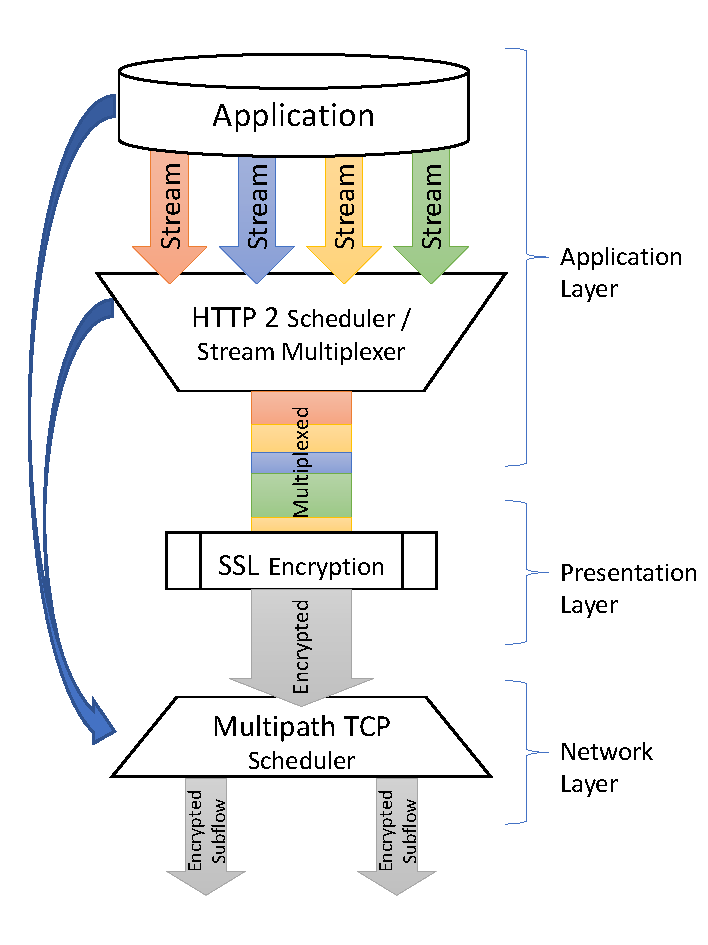
\includegraphics[width=0.4\textwidth]{mux-demux.pdf}
	\caption{Optimization across layers}
\end{wrapfigure}


% reasoning why mptcp is/will be used on devices people browse the internet with
Most smart phones and notebooks have multiple network interfaces nowadays. This has given rise to the design of various network protocols with the aim of extending bandwidth, enhancing reliability and lowering power consumption by intelligently combining interfaces. One of these is Multipath TCP  \cite{RFC6824_MPTCP}, an extension to the Transmission Control Protocol with support for combining multiple paths over multiple interfaces into a single TCP connection with higher bandwidth and reliability.


% users expect faster/instant reaction from computers/web pages/interactive services ^= do not accept (long) wait times
% web sites getting more complex
% 
% very short intro to mptcp, evtl. richtung vorteile f�r clients/webbrowsing
% ``more and more devices are mobile''
% ``almost every modern device has multiple network interfaces'' (smartphones cell+wifi, notebooks eth+wifi(+cell), desktops eth+wifi, household routers with multi uplink dsl+lte, etc)



Inherent in Multipath TCP operation is some overhead of discovering and establishing multiple paths when the connection is set up. In regular web browsing, HTTP up to version 1.1 use many short-lived TCP connections, so the overhead of multipath initialization can shatter the performance improvements of Multipath TCP, as the connection often is closed before the second path is usable. Combined with unadapted browsers, this can cause Multipath TCP to have worse performance than single path TCP \cite{han2015mwebmptcp}.


% very short intro to http/2, maybe difference to http/1(.1)
% ``websites become more intricate''
The web has come a long way since the introduction of HTTP/0.9 in 1993. Many small improvements have been made in the meantime, all carefully providing backward compatibility. But web applications have become so intricate, and users so accustomed to responsive interactive services, that a clear break had to be made. Therefore, HTTP/2 \cite{RFC7540_HTTP2} has been specified. To allow easier adaption, the semantics were kept intact, while the underlying protocol was changed completely: A only seemingly simple text-based protocol was replaced with a more efficient, precisely specified binary protocol. 
The new feature most relevant to us are multiplexed streams which allow all data to be transferred over few, long-lived, thus more efficient TCP connections. The multiplexing also prevents head-of-line blocking and allows prioritizing the most time-critical resources.

% two schedulers (
% - http2 schedules frames from multiple streams into one tls/tcp connection, mostly based on http2 priority;
% - mptcp schedules tcp segments from one meta socket onto multiple real sockets
% )
% three layers

As opposed to older versions, HTTP/2 is based on long-lived TCP connections. Therefore it can utilize the additional sub-flow capacity more often. During a single connection, different types of requests are processed, including loading a document and resources required to display it, loading auxiliary content like images below the fold, and user-initiated AJAX requests. Every type of request has different performance needs, which makes it especially interesting for cooperation-based optimization approaches.

% different scheduling approaches for mptcp are possible, many have been proposed and some are implemented in the linux kernel

% assumption: choosing best possible scheduling strategy depends on requirements of(/knowledge about/knowledge available to implementation of) higher level protocols 
% even for one given protocol, these requirements can change during a connection (e.g. web site: initial loading should be fast - user is waiting - use fastest flow(s)/use redundancy, loading of images below the fold don't need to be as fast -> conserve power/metered traffic, ajax requests might be small, but latency critical -> redundancy)
We assume that choosing the best possible Multipath TCP subflow scheduling strategy depends on information about the higher layers. In the case of HTTP/2 connections this information includes the type of the request as indicated above. For having this information available to the packet scheduler - part of the transport layer - there are several possible solutions, each coming with different pros and cons. 
% for some protocols, a good heuristical approach can be chosen based on transmitted bytes, time, transmission pauses, etc
For one, a heuristic approach can be chosen, which acts on metadata readily available in the transport layer, including transmission rate and pauses, elapsed time, and byte and packet counters. The good thing is that this approach is independent of the specific implementation of the application protocol, and can even work unchanged for several similar protocols. 
% for some protocols, the scheduler could look into the octet stream and decide depending on contents
% problems:
% -> breaks separation of layers - high ``dirty hack'' factor
% -> protocol decoding needs to be implemented in scheduler (os kernel!) -> proto updates need kernel updates, security problems (protocol parser is huge attack surface)
% -> impossible with encrypted protocols (not technically impossible, but would be very complicated and has performance hit)
Even more information about the state of higher level protocols can be gained by inspecting the octet stream itself. This brings with it all problems of Deep Packet Inspection, including security risks and increased code complexity \cite{Porter2005}. It is also not applicable to HTTP/2 as all browsers implement it with forced TLS encryption, therefore this approach is not considered any further.
% solution / our approach: the implementation of the higher level protocol provides special scheduling hints to the mptcp scheduler
% pro
% - no detailed knowledge about the protocol is neccessary in the scheduler
% - with a good api, the scheduler needs to know nothing about the specific application level protocol, while the app level proto implementation needs to know (almost) nothing about the network level scheduling
% contra
% - every application which should take advantage of this approach needs to be specifically modified
% - 
The middle road we suggest is providing an API which allows the application to provide scheduling hints to the transport layer. This has the advantage of not embedding knowledge about the application layer protocol in the scheduler, thereby keeping the abstraction layers separate.


%---------------------------------------------------------------------
\section{Approach}
%---------------------------------------------------------------------

%\todob{conceptual approach}
%wie vorgehen - konzeptioneller approach
%interaction / dependency -> l�sen durch cooperation
We start by analyzing the general structure of popular web sites regarding the resources on the critical path. In comparison, we look at guidelines for performance optimization in web design. 
From the gained insights, we conceive possible optimizations for existing, modified or specially crafted web pages at the transport level. The Multipath TCP implementation \cite{multipathtcp} consists of three major building blocks: path manager, packet scheduler and connection to the subflows \cite{RFC6182}. In this thesis, we pay special attention to the packet scheduler. More precisely, we concentrate on its component which spreads individual segments over subflows. These optimized schedulers are implemented in rule-based scripts which are loaded into the MPTCP implementation in the Linux kernel. To make scheduling hints like content type, priorities or dependencies available to the scheduler scripts, we modify a suitable HTTP/2-capable web server to pass on these hints as socket options. 

%auch implement. und eval approach
The next step is an evaluation of the implemented optimizations in simulated network environments. Web sites are loaded in network scenarios differing in bandwidth, round trip time and packet loss. To study the practicality, we conduct real-world measurements for the best-performing optimizations, connecting from LTE and domestic ADSL access networks to virtual servers at a cloud provider. 



%


%---------------------------------------------------------------------
\section{Structure}
%---------------------------------------------------------------------
% where we provide an overview of the chapters

% background/rel. work
In the following chapter, we introduce the protocols on which this work is based. This is Multipath TCP on the transport layer, which is described with a focus on scheduling. On the application layer, the HTTP/2 protocol and its underlying concepts. A review of related publications is conducted, with a focus on  Multipath TCP scheduling, coordination among software layers, cooperation between kernel and user-space components, web page optimization, and performance measurement of web pages and applications.

%approach
Chapter four starts with an analysis of typical web page structures, details our approach for passing scheduling hints from application to transport layer and presents optimized MPTCP scheduler rules for different network scenarios. We also consider security concerns regarding the scheduling hints as a side channel to TLS encryption.

%implementation
Following our approach of integrating multiple layers, the implementation described in chapter five ranges from the network layer up to the application layer. Optimized schedulers were realized with a scripting-enabled rule based scheduler in the Linux kernel. After conducting a survey of web server software, we choose one to customize. This is necessary to pass information about HTTP transactions down the stack, bypassing encryption. On top of that, we created sample web pages and applications.


%evaluation
To show which optimizations are worth using in which network situations, in chapter five, we evaluate the performance of the implemented schedulers in simulated and real-world networks. We conduct measurements including the resource usage, like transmitted data volume per interface, and record timestamps of all events in the browser, to calculate various page load speed metrics. Based on that data, we relate the added value for the user to potential computational overhead and bandwidth costs.


%their actual and perceived speed, utility to the user, overall and per-interface bandwidth usage, (power usage?), computational overhead, implementation difficulty, 

%conclusion
Finally, a conclusion is drawn on the accomplished improvements, which approaches were successful and which less so. We also use the last chapter to point out possible future work.


%problem statement

% analysis of the possible ways for interaction between transport and application layer in the case of MPTCP and HTTP2

% analysis of typical web page structures

% design and implementation of MPTCP scheduler(s) for optimizing web page loading / web app usage, which get (out of band) information from presentation layer TLS, application layer HTTP2 and/or  application layer HTML, JS,... (Web Page Structure)

% evaluation of the optimizations





%=====================================================================
\chapter{Background and Related Work}
%=====================================================================

%related work
In this chapter, we go through transport, presentation and application layer, the OSI layers this work is concerned with. For each layer, we explain the relevant protocols and implementations. We will also present previous work on the optimization and measurement of web page performance.


\section{Transport Layer: Multipath TCP}

%
%http://www.ip-insider.de/anwendungen-und-konkurrenz-fuer-multipath-tcp-a-445245/
%\cite{IpInsiderMptcp}

Two pipes are better than one - that's Multipath TCP in a nutshell. In this case, a pipe is a distinct path between two devices, identified by the IP adresses of both peers. Combining multiple of these subflows can provide several advantages. Higher throughput can be achieved by multiplexing data over multiple subflows. The reliability of a connection can be improved by establishing backup subflows: in case a subflow stops working, the backup takes over seamlessly. On routes with packet loss, the latency can be reduced by sending packets redundantly on multiple subflows. 

This section covers the background knowledge on Multipath TCP which is required for the remaining work. We start by enumerating the current software implementations of Multipath TCP and giving some information on its current deployment. Following that, we describe the architecture of protocol and implementations. We present studies evaluating and optimizing Multipath TCP performance, and proposals and implementions of interfaces to the application layer. To finish this section, we explain the rule-based scheduler, a Multipath TCP packet scheduler, which makes its decisions based on script programs which are changeable during runtime, allowing us to evaluate different scheduling approaches faster.

%tuple of (source address, source port, destination address, destination port).


% multiple network interfaces
\begin{table}%
		\begin{tabular}{ll} \toprule
		Device Type    & Network Interfaces \\ \midrule
		smart phones & Wi-Fi and cellular \\
		notebooks & Wi-Fi, often Ethernet, sometimes cellular \\
		desktops & Ethernet and/or Wi-Fi \\
		servers & multiple Ethernet \\
		household routers with multiple uplinks & DSL and cellular (LTE) \\ \bottomrule
		\end{tabular}
		\caption{Typical network interfaces of common device types}
		\label{}
\end{table}


\subsection{Implementations and Deployment}
%We start by enumerating the current software implementations of Multipath TCP and giving some information on its current deployment.

%reference(?) implementation in linux kernel
The current reference implementation\footnote{\url{http://multipath-tcp.org/}} is based on the Linux kernel and maintained by \textcite{multipathtcp} at the Universit� Catholique de Louvain. A similar patch for the FreeBSD kernel has been developed at Swinburne University\footnote{\url{http://caia.swin.edu.au/newtcp/mptcp/}}.
%https://support.apple.com/en-us/HT201373
 The first implementation of Multipath TCP was developed as a user-space proxy\footnote{\url{https://open-innovation.alcatel-lucent.com/projects/mptcp-proxy}} by Hampel at Bell Labs, and is no longer maintained. All aforementioned software is open source. There is also one known closed-source implementation by Citrix Networks in their load balancer firmware \cite{Eardley2013}.
%other implementations
The most widely deployed implementation is found in Apple's XNU kernel \cite{Hesmans2016}, used in the macOS and iOS operating systems. It is used mainly for the Siri personal assistant software, which keeps a backup connection over cellular network in case the Wi-Fi connection breaks down \cite{AppleSupportMPTCP}. 
\textcite{Bonaventure2016Deploy} report a similar use by some cellular network operators. Hardware vendors include the Multipath TCP implementation in the Linux kernel of their Android phones. The cellular provider provides a SOCKS proxy server at carrier level. Together with a SOCKS proxy in the Android operating system, both using Multipath TCP, this allows combining Wi-Fi and cellular connectivity over existing infrastructure. 


\subsection{Architecture of Multipath TCP}
%Following that, we describe the architecture of the Multipath TCP protocol and implementation. 

\begin{figure}
	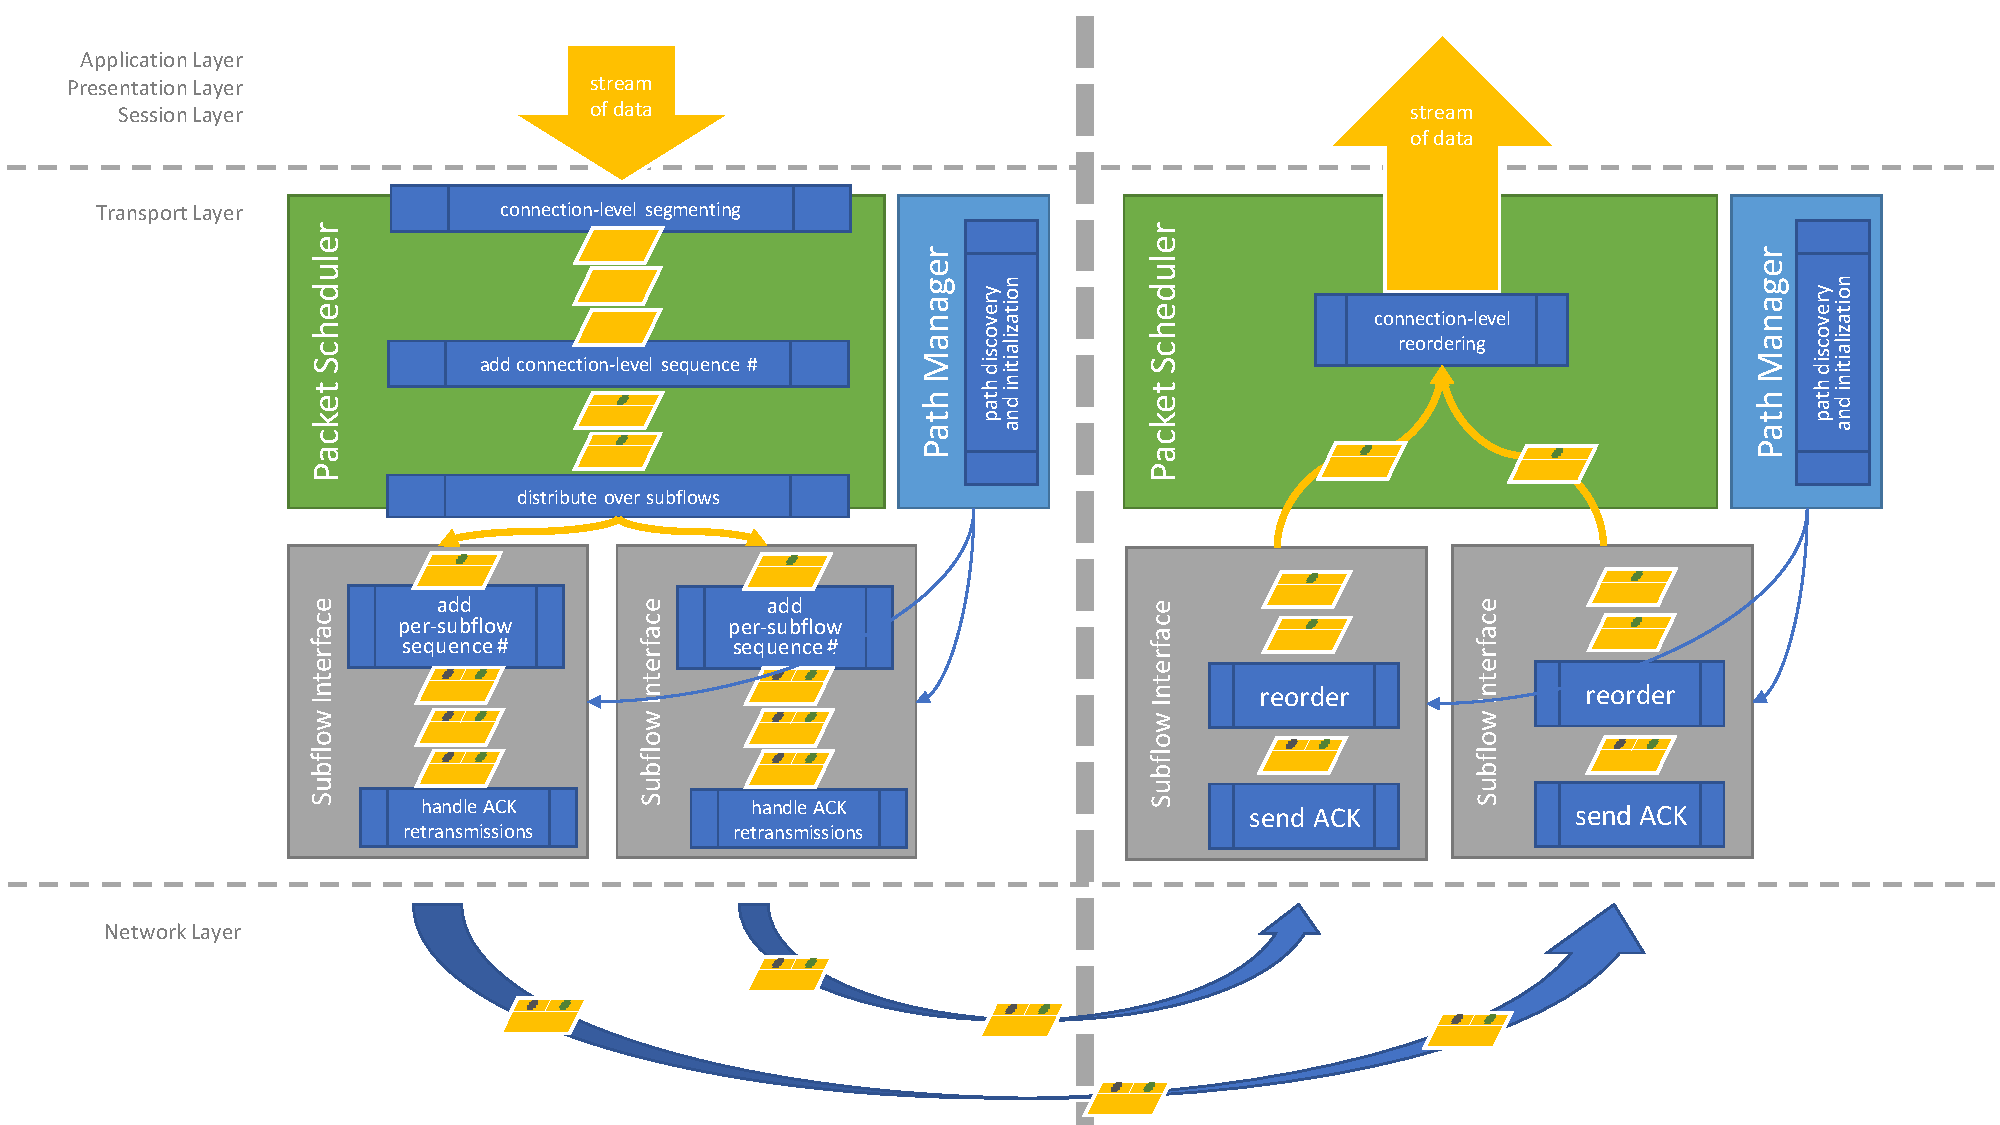
\includegraphics[width=0.9\textwidth]{mptcp-functional-decomposition.pdf}
	\caption{Interaction of the functional building blocks of Multipath TCP as described in \cite{RFC6182}}
\end{figure}

%\subsubsection{Path Management}



%\subsubsection{Packet Scheduling}




%\subsubsection{TCP Subflows}


\subsection{Multipath TCP on the Wire}

Great care was taken in the specification of Multipath TCP to maintain compatibility with regular TCP, not only but especially towards the network layer. This was done with regard to the deploying it in the current Internet, which means coping with network address translators, firewalls and other middleboxes.
Therefore, Multipath TCP subflows look and behave on the wire exactly like regular TCP flows, except the segments contain some additional TCP options as described in RFC 6824 \cite{RFC6824_MPTCP}.

When a new Multipath TCP connection is set up, the \textbf{MP\_CAPABLE} option is included in the SYN segment. From this options, the server learns that the new client supports MPTCP. In the responding SYN-ACK and ACK segments, the MP\_CAPABLE option is included as well, serving as a handshake, in which authentication keys are exchanged. These keys are later used in the process of adding more subflows to the connection.

New subflows are initiated by establishing what looks like a regular TCP connection at to the network, but contains the \textbf{MP\_JOIN} option in the three-way handshake segments. The contents of this option depends on the stage of the handshake. The initiator sends an identifying token, which is based on the authentication keys.  In the first two segments, random numbers (nonces) are exchanged. To authenticate each other, the peers exchange HMACs of the concatenated nonces keyed on the concatenated authentication keys in the second and third segment.

During the regular data transmission, the \textbf{DSS} option (Data Sequence Signal) is added to every segment. It contains sequence numbers and acknowledgements, which work very similar to their TCP counterparts. They are necessary to ensure ordered data transfer across subflows, and to retransmit segments in case of collapse of a subflow.


\subsection{Performance Evaluations}
%We present studies evaluating and optimizing Multipath TCP performance, [...]



\subsection{Socket API}
%We present [...] proposals and implementions of interfaces to the application layer.

%application api's
The only way to control the current Linux implementation from user-space was by setting \code{sysctl} parameters, which are generally valid for the entire operating system. They allow the system administrator to enable or disable Multipath TCP for all applications, and to change a number of high-level parameters globally. If Multipath TCP is enabled, it is used for all TCP connections and is transparent to the application. Recently, the socket option \code{MPTCP_ENABLED} was introduced, which allows switching it on or off per socket. Still, application developers don't have any fine-grained control over the Multipath TCP behaviour.

In contrast, the Apple implementation takes a very different approach by providing a new socket-based API. One the positive side, this gives Multipath TCP aware applications full control over Multipath TCP connections, setting up, enumerating and tearing down subflows. New \code{connectx} and \code{disconnectx} system calls are introduced for that reason. However, this makes it incompatible to existing applications, requiring developers to make modifications to take advantage of the new protocol.

To allow similar fine-grained control, while keeping the compatibility with unadapted applications, several APIs have been proposed. 
%RFC 6897
\textcite{Scharf2013} present in RFC 6897 a ``Basic API for MPTCP-Aware Applications'', enabling applications to restrict the interfaces to use for establishing paths and to query the subflows and their addresses. 
They also recommend that socket options on a Multipath TCP meta-socket should be, if possible, passed through to all subflow sockets.
%Hesmans 2016 - An enhanced socket API for Multipath TCP




\subsection{Optimizing Multipath TCP Scheduling}



\subsection{Rule-Based Scheduler}
The rule-based scheduler by \textcite{RBS} is a Multipath TCP scheduler, which runs a small program for every scheduling decision. These programs can be written in a special scripting language and are compiled to a byte code, which is executed by a virtual machine in the scheduler. The possibility of dynamically loading the scheduling algorithms at runtime, without having to recompile the Linux kernel, allows us to evaluate different scheduling approaches quickly.

%cf implementation: The scheduler algorithms are implemented in a scripting language. The scripts are just-in-time compiled and interpreted by the Rule Based Scheduler, a byte-code based virtual machine running in the MPTCP implementation in the Linux kernel.


% subflow attributes
\begin{table}
	\begin{tabularx}{\linewidth}{ l X } \toprule
	Attribute & Description \\ \midrule
	\texttt{ID}								& Numeric identifier of the subflow. Unique per MPTCP connection. \\
	\texttt{RTT} 							& Calculated round trip time on this subflow in milliseconds. \\
	\texttt{LOST\_SKBS} 				& Number of packets which were lost on this subflow. \\
	\texttt{SKBS\_IN\_FLIGHT} & Number of packets which were sent out on this subflow but not yet acknowledged or retransmitted. \\
	\texttt{CWND} 						& Congestion window. Number of packets which are allowed to be in flight on this subflow at the same time. \\
	\texttt{IS\_BACKUP} 			& Boolean flag, set to \texttt{1} if subflow is marked as a backup subflow by the user or operating system. \\
	\bottomrule
	\end{tabularx}
	\caption{Information about a subflow available to the MPTCP scheduler}
	\label{}
\end{table}


\section{Presentation Layer: SSL}

% why we need to consider ssl
% - x% of connections use ssl today
``In September 2014, 44.3% of web connections already use HTTPS.''
``The growth of HTTPS adoption is striking, with the HTTPS ?ow share more than doubling in two years.''
``the �S� is here to stay''

OpenSSL will build a record from each call to�SSL\_write
https://www.imperialviolet.org/2010/06/25/overclocking-ssl.html



``the TLS standard provides a fast negotiation mechanism, which reduces the TCP+TLS handshake to 2 RTTs�'' (session id)


\section{Application Layer: HTTP/2 and HTML}

The HyperText Transfer Protocol (HTTP) is the protocol which is used by web browsers to load web sites from web servers. But since its inception in 1993, web sites have changed a lot, which caused the need for improvements in HTTP. For example, modern web sites often consist of hundreds of individual files. With classic HTTP/1.0, a new TCP connection is established for every file, which needs three round trips. If encryption is used, an individual TLS handshake is performed as well, which needs another four round trips. To improve the situation, connection keep alive was introduced with HTTP/1.1, an extension which allows to use the same connection for multiple downloads. 
Another problem is the verbosity of HTTP/1's text-based protocol. The meta data (HTTP header) is transmitted as human-readable text, which makes debugging easier, but uses more bandwidth and is more complex to parse. There have been approaches at compressing the headers, but this caused security problems and was therefore not 
The web has come a long way since the introduction of HTTP/0.9 in 1993. Many small improvements have been made in the meantime, all carefully providing backward compatibility. But web applications have become so intricate, and users so accustomed to responsive interactive services, that a clear break had to be made. Therefore, HTTP/2 \cite{RFC7540_HTTP2} has been specified. To allow easier adaption, the semantics were kept intact, while the underlying protocol was changed completely: A only seemingly simple text-based protocol was replaced with a more efficient, precisely specified binary protocol. 
The new feature most relevant to us are multiplexed streams which allow all data to be transferred over few, long-lived, thus more efficient TCP connections. The multiplexing also prevents head-of-line blocking and allows prioritizing the most time-critical resources.


As opposed to older versions, HTTP/2 is based on long-lived TCP connections. Therefore it can utilize the additional sub-flow capacity more often. During a single connection, different types of requests are processed, including loading a document and resources required to display it, loading auxiliary content like images below the fold, and user-initiated AJAX requests. Every type of request has different performance needs, which makes it especially interesting for cooperation-based optimization approaches.


%``HTTP/2 is a binary, rather than text, protocol, making it more compact and efficient
%It uses a single, multiplexed connection per domain, rather than multiple connections carrying one file each
%Headers are compressed with the purpose-built HPACK protocol (rather than gzip, as in SPDY)
%HTTP/2 has a complex prioritization scheme to help browsers request the most-needed files first, which is fully supported in NGINX (SPDY had a simpler scheme)''
%https://www.nginx.com/blog/7-tips-for-faster-http2-performance/


\subsection{Optimizing HTTP}
(web performance? http2 performance?)
\cite{klotski2015}
(general article about HTTP/2 as optimization of http)
\cite{RFC7540_HTTP2}

\subsection{Streams}

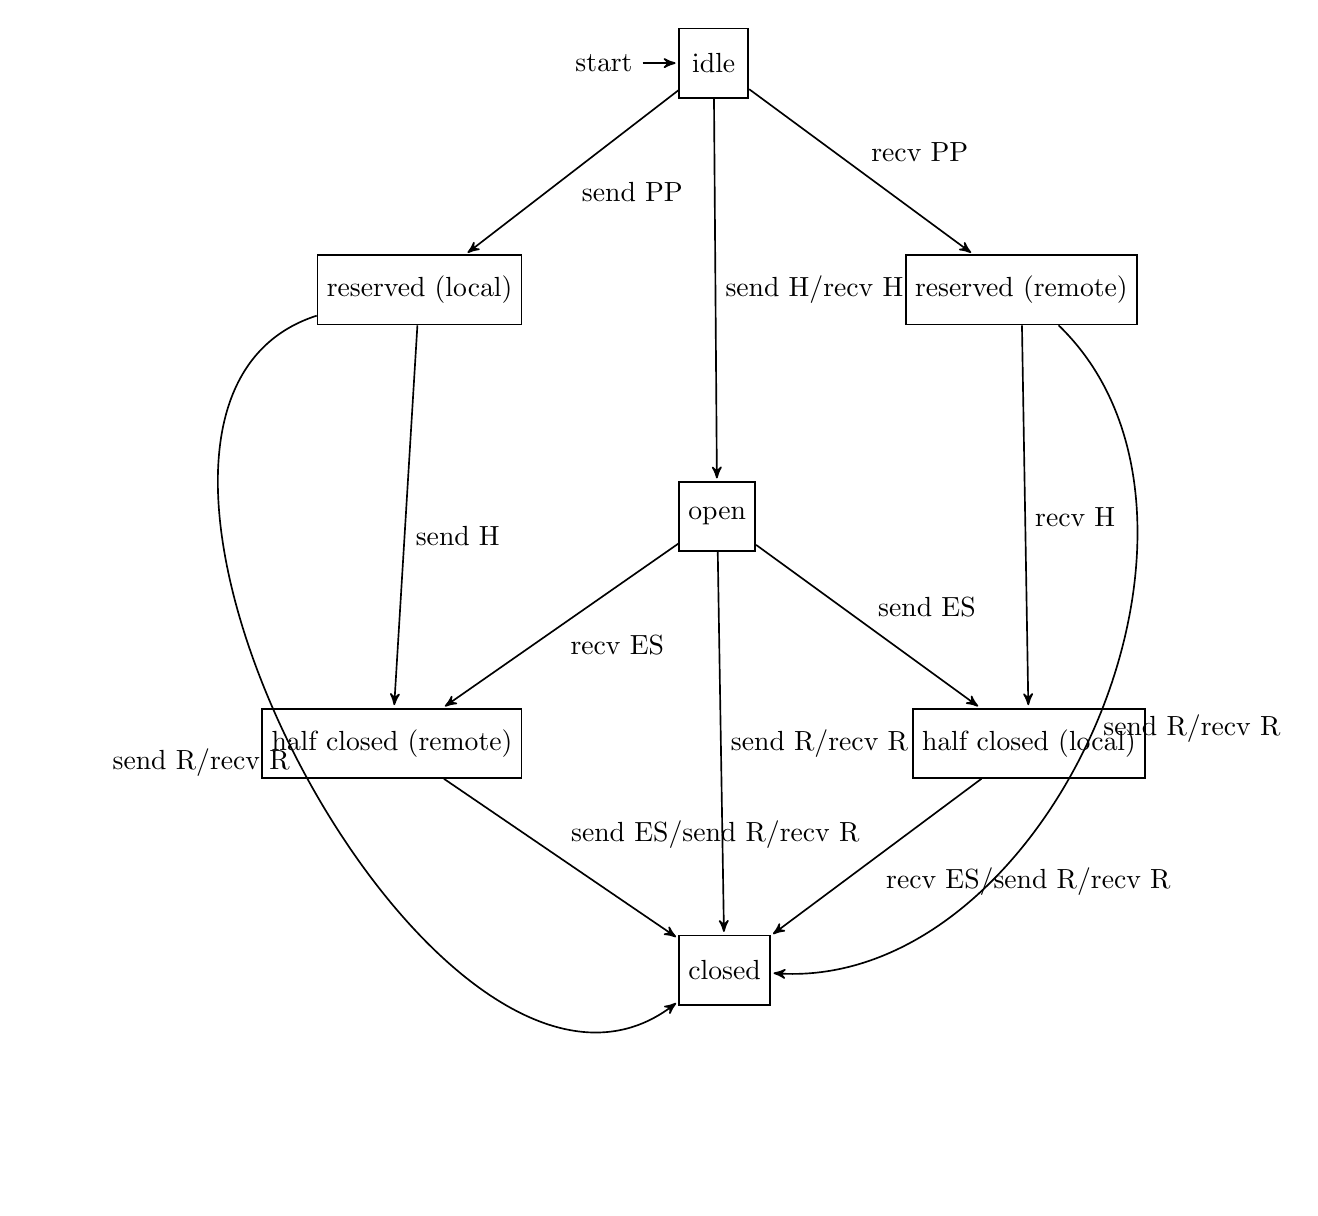
\begin{tikzpicture}[->,>=stealth',shorten >=1pt,auto,node distance=2.8cm,
	semithick]
	\tikzstyle{every state}=[draw, rectangle]

	\node[initial,state](idle){idle};

	\node[state, below left =of idle](rsv_loc){reserved (local)};
	\node[state, below right= of idle](rsv_rem){reserved (remote)};
	\node[state, below right =of rsv_loc](open){open};

	\node[state, below left=of open](hc_rem){half closed (remote)};
	\node[state, below right=of open](hc_loc){half closed (local)};

	\node[state, below right=of hc_rem](closed){closed};


	\path (idle) edge node {send PP} (rsv_loc)
	(idle) edge node {recv PP} (rsv_rem)
	(idle) edge node {send H/recv H} (open)
	(rsv_loc) edge [bend right=100] node[left] {send R/recv R} (closed)
	(rsv_rem) edge [bend left=70] node[right] {send R/recv R} (closed)
	(rsv_loc) edge node {send H} (hc_rem)
	(rsv_rem) edge node {recv H} (hc_loc)
	(open) edge node {recv ES} (hc_rem)
	(open) edge node {send R/recv R} (closed)
	(open) edge node {send ES} (hc_loc)
	(hc_rem) edge node {send ES/send R/recv R} (closed)
	(hc_loc) edge node {recv ES/send R/recv R} (closed)
	;

\end{tikzpicture}

http://http2.github.io/http2-spec/index.html\#StreamStates


\section{Performance of Web Traffic on Multipath TCP}


%HTTP/1.1 mostly benefits from Multipath TCP for larger file downloads because the TCP connections are often closed after one download, whereas the overhead of establishing auxilliary paths is not worthwile for downloading only one small file. In some studies it has been shown that the HTTP/1.1 performance is worse with MPTCP that with single path TCP on the same connection. Especially the common HTTP/1.1 optimization practice of sharding (spreading files among many different origins).
 
Inherent in Multipath TCP operation is some overhead of discovering and establishing multiple paths when the connection is set up. Older versions of HTTP use many short-lived TCP connections, so the overhead of multipath initialization can shatter the performance improvements of Multipath TCP. Combined with unmatched expectations of the browser, there are situations where Multipath TCP can hurt the HTTP/1.1 performance compared with single path TCP \cite{han2015mwebmptcp}.



\section{Measuring Web Performance}
\cite{han2015mwebmptcp}

%	1. PageLoadTime (Zeit bis Load Event)
%	2. Zeit bis DOMContentLoaded Event
%	3. First Paint / First Contentful Paint / First Meaningful Paint
%	> First Meaningful Paint is essentially the paint after which the biggest above-the-fold layout change has happened, and web fonts have loaded. See the spec to learn more: First Meaningful Paint: A Layout-Based Aproach.
%	https://developers.google.com/web/tools/lighthouse/audits/first-meaningful-paint
%	``Time to First Meaningful Paint: A layout-based approach''
%	https://docs.google.com/document/d/1BR94tJdZLsin5poeet0XoTW60M0SjvOJQttKT-JK8HI/view#heading=h.tdqghbi9ia5d

%1 und 2 sind �ber chrome remote debugging api leicht erh�ltlich (Page.loadEventFired)
%3 ist im Devtools Timeline view sichtbar, muss also auch �ber das remote debugging api verf�gbar sein (Devtools verwenden selber auch das rda)

%Chrome Debugging - Tracing
%https://chromedevtools.github.io/debugger-protocol-viewer/tot/Tracing/
%https://docs.google.com/document/d/1CvAClvFfyA5R-PhYUmn5OOQtYMH4h6I0nSsKchNAySU/edit



\subsection{Categorizing web page components}

%Automatische Einstufung von Seitenbestandteilen (HTTP Requests) in Relevanz / User Utility
%-> nicht Thema der Arbeit, aber evtl. relevant f�r praktische Umsetzung

%Automatisches Aufbauen von Dependency Graphs


\section{Cooperation of Application Layer and Transport Layer}

% technical problems to be solved:
% *api needs to be defined
% *there might be a layer in between (Presentation Layer, TLS omnipresent today)

There are two main technical challenges in cooperation between (network) layers:

The first is that an adequate API needs to be defined. This is tricky especially in our case, the cooperation of application and transport layer, as one side is in user space and the other is a kernel component in modern operating systems.

The second challenge results from the fact that these layers are not directly adjacent to each other: In our case it is TLS encryption, which operates in the presentation layer, making all application layer data opaque to layers below. Therefore, a side channel needs to be established to allow information flow around the TLS encryption.
% see also: security considerations...


% research: what kinds of information that one layer has available, could provide an advantage to an other layer

research: what kinds of information that one layer has available, could provide an advantage to an other layer

\cite{Raisinghani_2004}
\cite{nowlan2012unorderedtcp}




%=====================================================================
\chapter{Approach}
%=====================================================================


	
%Annahmen:
We will describe a few assumptions made for the implementation and all optimizations.
%TCP-Verbindung wird immer vom Browser aufgebaut
First, we always look at a MPTCP connection which is established by the web browser and accepted by the web server. This is always the case for HTTP connections.
%Nur der Client/Browser hat mehrere Interfaces / sendet MP JOIN Anfragen -> path-manager erstmal nicht relevant
Only the client has two interfaces with different network addresses. After the connection is set up, it directly opens the second subflow by connecting to the server from the secondary interface with a \code{MP_JOIN} option in the \code{SYN}. The server has only one (visible) interface and accepts the second subflow. Therefore we won't discuss different MPTCP path management algorithms.
%Client hat zwei Interfaces (Wi-Fi und 3G)
The client's interfaces are either Wi-Fi and 3G/LTE, as found on smart phones, or Ethernet and Wi-Fi, which is common for notebooks.
%Kontrollierbare Aspekte: 
%	- Scheduler
%	- TCP Flow Control/Congestion Control




\section{Analysis of web page behaviour}



\section{Interaction between transport and application layer}

%Wie dem Scheduler mitteilen was er tun soll?
%Problem: Wie erfolgt Kommunikation mit dem mptcp-scheduler? Zwischen mptcp und http2 sitzt in der regel noch tls! -> Paketinhalt f�r mptcp-scheduler nicht lesbar - evtl. �ber byte-counter


%Wo kommt die Logik hin?
%	- a: Server taggt Frames irgendwie, z.B. Inhalt=PageContent / Bild / Script / Style; Push=Ja/Nein; etc�, und Scheduler enth�lt die Logik die sagt was mit welchem Frame-Typ passieren soll
%oder b: Server gibt genaue Anweisung an Scheduler, dieser setzt es nur um
A decision we need to make is where to place the optimization logic. One approach is that the server tags every HTTP/2 frame with information like content or stream type, and the scheduler script decides that to do exactly. This way, there is maximum flexibility for the MPTCP configuration and the server doesn't need to know very much about MPTCP. On the other hand, we need special handling on the scheduler level for every application protocol we want to optimize.
The other approach is to have several general scheduler algorithms, each with different performance trade-offs, while allowing the application to decide which scheduler algorithm should be enabled. This reduces the dependencies on the scheduler level, but required more MPTCP specific decision making on the application level. 





\section{Optimizing the Multipath TCP scheduler}

Several optimization approaches are considered in this chapter.

\subsection{Switching the scheduler based on content type or priority}
Many modern web pages consist of dozens of resources. They can be classified by their technical priority for rendering the page. 

1. The \textit{Document} is the main HTML file which is loaded first. It is strictly necessary for the browser to render the page, and to load subsequent resources. 

2. Synchronous Javascript resources (\code{<script>} tags) are required by the browser to construct the Document Object Model (DOM) tree. They must be loaded as soon as the tag is parsed by the browser.

3. Style sheets are needed for the first layout cycle of the page, which means usually nothing is displayed to the user until they are fully loaded.

4. Images can be loaded after the base frame of the site is visible, especially if the image size is provided in the Document source. The same is true for video, audio and most AJAX requests.

...

One can also look at their subjective utility to the user.

In the case of text heavy pages, like news sites, the Document and some images are most useful to the user as that contains the content of the page. In these cases, the Javascript resources are often providing tracking and advertising, so very important for the webmaster but annoying for the user. Especially tracking scripts can be delivered with lower priority as they are invisible and not time critical.

For interactive pages, the Javascript might provide all the relevant contents.   

...  ... 

Modern browsers and speed-optimized web pages make sure that the resources with the highest technical priority are requested first. The HTTP/2 server can also facilitate this by pushing out high-priority resources with HTTP Push.

The resources required for the first layout cycle will be handled by a scheduler with emphasis on low latency, like a redundant scheduler on lossy connections. The redundant scheduler sends all segments out on all paths to minimize delays caused by packet loss.

After these high priority resources are sent out, a regular, more bandwidth conserving scheduler can be used.



\subsection{Aggressive transmission of last segments}
The transmitting application signals the state of its outgoing buffers to the scheduler. An interesting condition occurs when the HTTP server has no more data to send, and only a few segments are left in the scheduler's queue. This means only these few segments are missing so that a complete web page can be rendered for the user. The scheduler can try to push out the missing segments more aggressively: By temporarily ignoring the available congestion window for the left over bytes, or by retransmitting on all available subflows.





\section{Security Considerations}
The information passed from the HTTP server to the MPTCP scheduler creates a side channel bypassing TLS encryption. It needs to be considered whether the passed data or the observable scheduler decisions based on this data could help an adversary. Some information are only protected by HTTP/2 and would be exposed on HTTP/1.1 connections anyway, like the length of individual resources. Others, like the content type, might be not available to the attacker otherwise.






%=====================================================================
\chapter{Implementation}
%=====================================================================


\begin{figure}[b]
	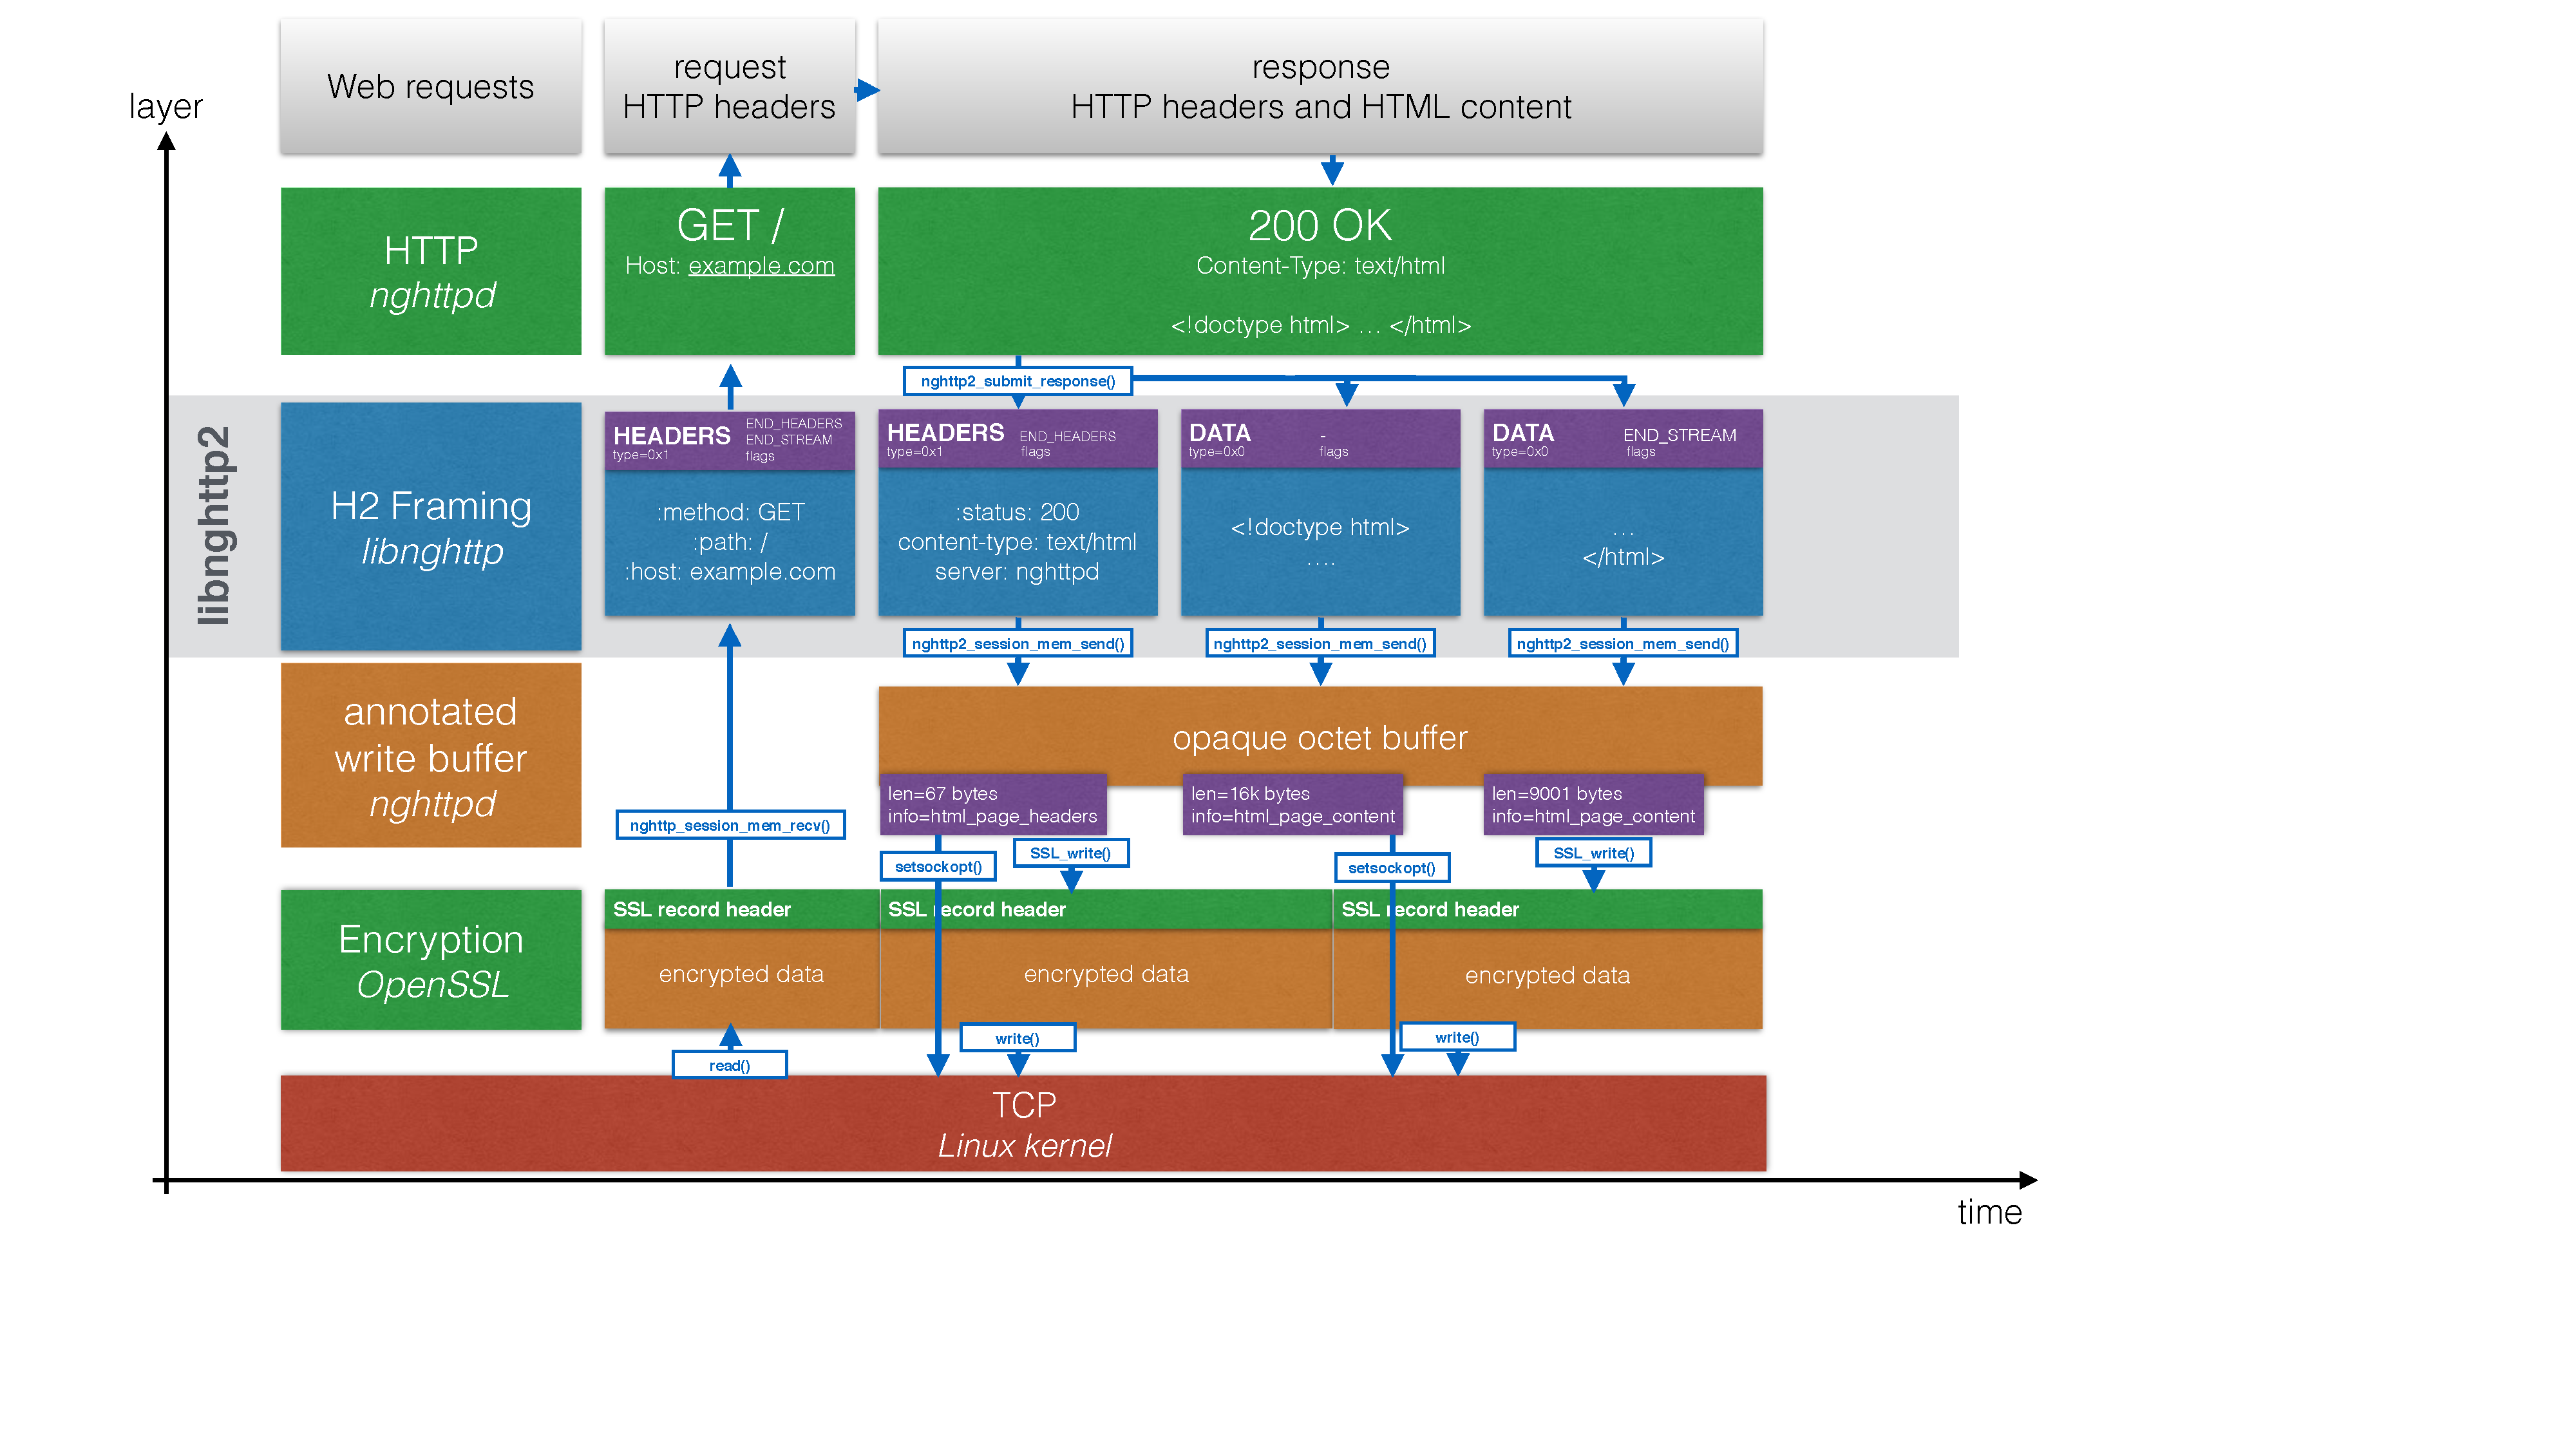
\includegraphics[width=1\textwidth]{http2-awb-layers.pdf}
	\caption{The annotated data's path through the application and network layer}
\end{figure}


\section{Transport Layer: Multipath TCP}

\subsection{TCP}


\subsection{Scheduler}


The scheduler algorithms are implemented in a scripting language. The scripts are just-in-time compiled and interpreted by the Rule Based Scheduler, a byte-code based virtual machine running in the MPTCP implementation in the Linux kernel.



\subsection{Socket Buffers}





\section{Application Layer: HTTP 2}


\subsection{Choosing a web server platform}

To get information about the contents of the HTTP/2 application data, the cooperation of the web server is required.

Multiple web servers have been evaluated and based on the criteria set out below, a suitable implementation basis has been selected.

As we want to implement low-level modifications in the web server, the source code has to be available, and the license must permit modifications. This is a strictly necessary criterion, but luckily, most available web servers are permissively open source licensed under Apache, MIT or similar licenses.

To be at all useful, the server must support HTTP/2, and support it with at least one common browser as client. 

To make the work more relevant for practical use, a popular web server should be used. Therefore, we started our evaluation with the Apache HTTP Server


\subsubsection{nghttpd}

.....

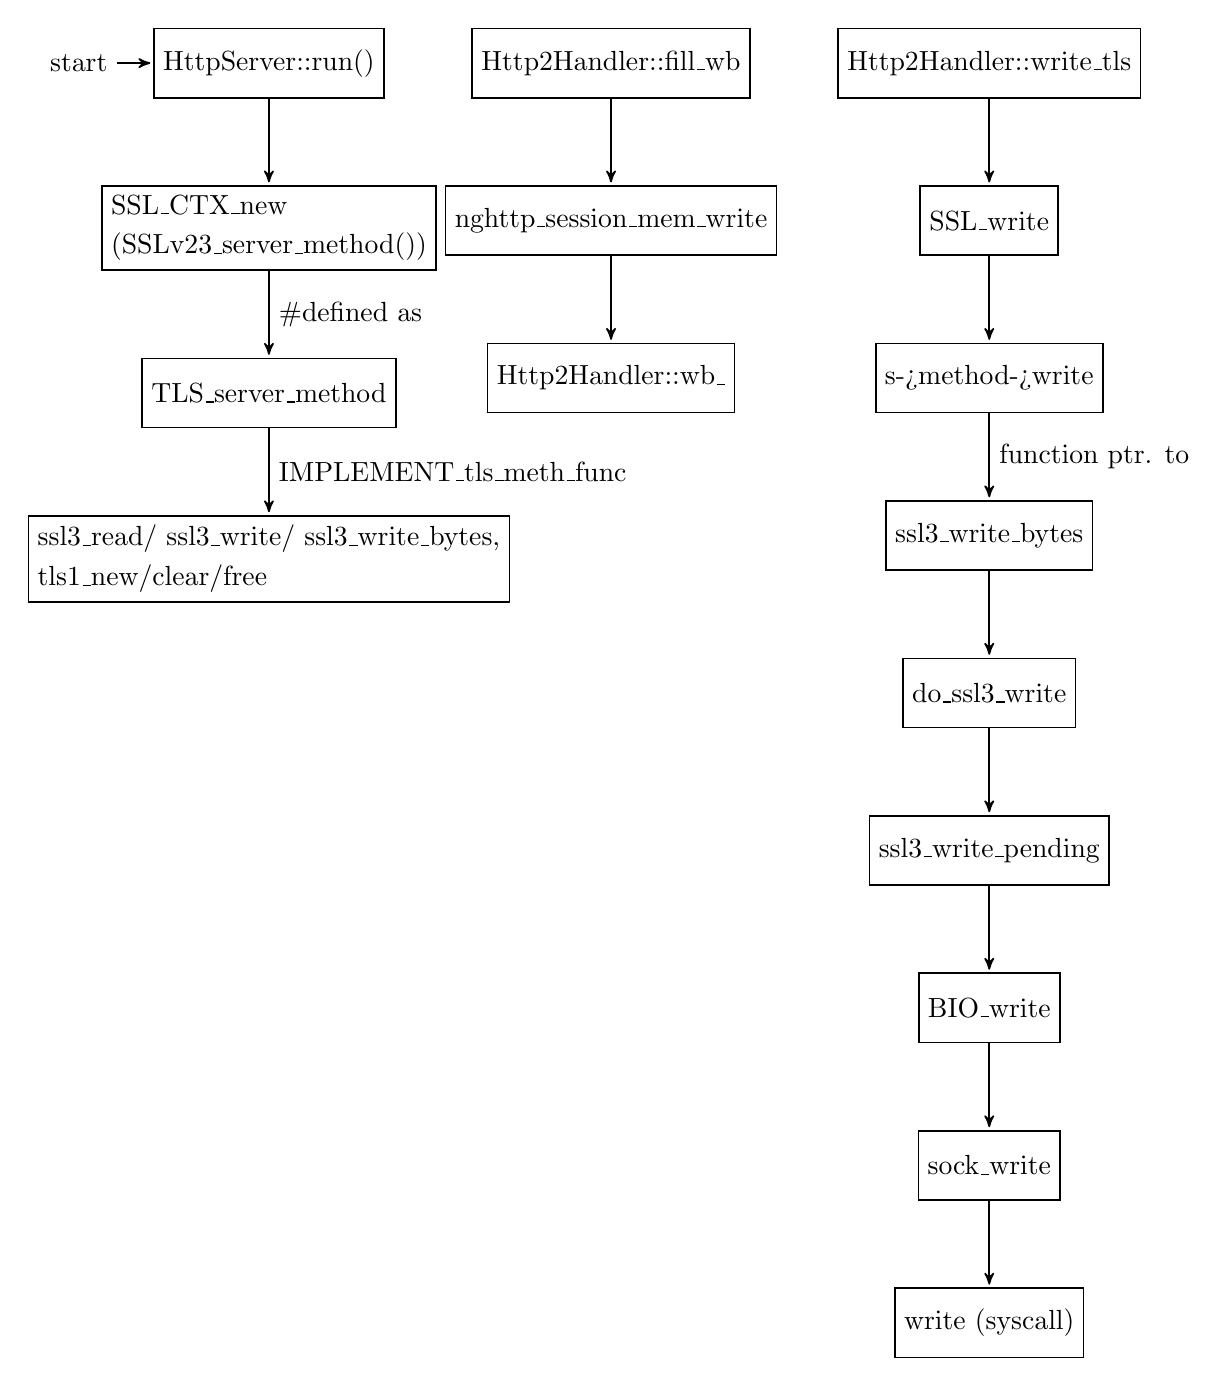
\begin{tikzpicture}[->,>=stealth',shorten >=1pt,auto,node distance=1.1cm,
		semithick]
	\tikzstyle{every state}=[draw, rectangle,
	execute at begin node={\begin{varwidth}{21em}},
	execute at end node={\end{varwidth}}]

	\node[initial,state](s1){HttpServer::run()};
	\node[state,below=of s1](s2){SSL\_CTX\_new \\(SSLv23\_server\_method())};
	\node[state,below=of s2](s3){ TLS\_server\_method  };
	\node[state,below=of s3](s4){ ssl3\_read/ ssl3\_write/ ssl3\_write\_bytes, tls1\_new/clear/free };


	\node[state,right=of s1](s6){  Http2Handler::fill\_wb };
	\node[state,below=of s6](s7){  nghttp\_session\_mem\_write };
	\node[state,below=of s7](s8){  Http2Handler::wb\_ };



	\node[state,right=of s6](s9){  Http2Handler::write\_tls };
	\node[state,below=of s9](sa){  SSL\_write };
	\node[state,below=of sa](sb){  s->method->write };
	\node[state,below=of sb](sc){  ssl3\_write\_bytes };
	\node[state,below=of sc](sd){  do\_ssl3\_write };
	\node[state,below=of sd](se){  ssl3\_write\_pending };
	\node[state,below=of se](sf){  BIO\_write };
	\node[state,below=of sf](sg){  sock\_write };
	\node[state,below=of sg](sh){  write (syscall) };

	\path (s1) edge (s2)
	(s2) edge node {\#defined as} (s3)
	(s3) edge node { IMPLEMENT\_ \\ tls\_meth\_func} (s4)

	(s6) edge (s7)
	(s7) edge (s8)

	(s9) edge (sa)
	(sa) edge (sb)
	(sb) edge node {function ptr. to} (sc)
	(sc) edge (sd)
	(sd) edge (se)
	(se) edge (sf)
	(sf) edge (sg)
	(sg) edge (sh)
	;


\end{tikzpicture}




%=====================================================================
\chapter{Evaluation}
%=====================================================================

We start this chapter by a presentation of the evaluation setup and the reasoning behind the choices. This includes the software used, the data points collected, and the web sites to test the optimizations on.
Thereafter, the gathered data is presented and analyzed.


% overview of the chapter

% 1. decisions we made which have an impact on the evaluation:
%  -- using real web sites / hand-crafted sample web sites
%  -- if real web sites: which web sites to measure, how to prepare them for measurement
% - evaluation setup:
%  -- which browser to use for measurement
% - measured data points:
%  -- amount of data transmitted (overall, per interface/subflow)
%  -- complete page load time (onLoad)
%  -- load time of HTML Document
%  -- time to DOM Ready (doc + blocking scripts)
%  -- time to first render/paint
%  -- time to ``above the fold ready'' (this is probably the closest to user impression of load time)
%     - can be measured as the time of the last change above the fold
%  -- time to ``text ready'' (useful e.g. on newspaper sites where most users want to read the content only/first, but lot of slow crap is shown above the fold)

% 2. how the measurement is conducted (used browser, used additional scripts/extension to gather data from browser, additional scripts to gather transmitted data from network stack client/server side, automation, ...)
% -> this could as well go into Implementation???

% 3. results: data, graphs, observations, conclusions...









\section{Selection of sample web pages}

We have to decide which web sites to measure.

- Synthetic content / Self built test pages (plain html, small html file with many scripts/css, big html, etc ...)


Measuring the page load times of real-world web pages (mirrored on special web server under our control. Mirroring is necessary for multiple reasons: First, to ensure repeatability of the results we don't want the load of the ``real'' web server and the network connection in between to compromise our measurement. Second, we need the web server to support HTTP/2, which is not too common, and MPTCP, which is extremely rare in the wild)

- Alexa Top Sites (or similar ranking)

- Hand-selected sites with interesting features / problems / optimization potentials

- Sites which are often used on mobile



\section{Preparation of real-world web sites}

Some real-world web sites can be used as is for evaluation by using the ``Save as'' option of a web browser. This is especially true for web sites with no content loaded with JavaScript and no third-party content.
Most web sites need to be prepared in one or another way. Changes are inevitable when sites won't work otherwise. This is the case if the site is usually loaded over unencrypted HTTP, as for HTTP/2, browser enforce the use of TLS encryption. For third-party content, various possible solutions are discussed below.
There are sites which we can test unmodified, but where we should change things to get more realistic results. For example, many sites use special optimizations which are tailored to HTTP/1.1, which make things worse on HTTP/2. This is the case for sharding\footnote{\url{https://www.nginx.com/blog/7-tips-for-faster-http2-performance/\#tip7sharding}}
% web sites need to be prepared
% some can be used as is
% on some, changes are inevitable, they won't work otherwise (https neccessary for h2, problems with third-party requests and dynamic content, etc)
% on some, we should change stuff, e.g. because there are optimizations for http/1.1 which make things worse on http/2 and it would be unrealistic to use them in this state
% etc.



\subsection{Handling dynamic and third party requests}

Downloading web pages with browser / wget and delivering with nghttpd - Problem: how to handle dynamic or third-party requests?

\begin{itemize}
	\item Cancel/reject all third party requests (in-browser / iptables)

	Pro: Easy, reproducible

	Con: not realistic (always a lot faster than real request)

	Pro: might be faster by the same amount, so still comparable (?)

	\item Let all third party requests through to the original sites

	Pro: Easy, realistic

	Con: dependent on network condition of test computer and load on original server (not reproducible)

\end{itemize}

Alternative: Use a caching HTTP/2 proxy (nghttpx, apache)

Pro: realistic (?), reproducible, (not that difficult either)

Con: ...


\section{Metrics For Evaluation Of Web Performance }

\begin{wrapfigure}{r}{0.45\textwidth}
	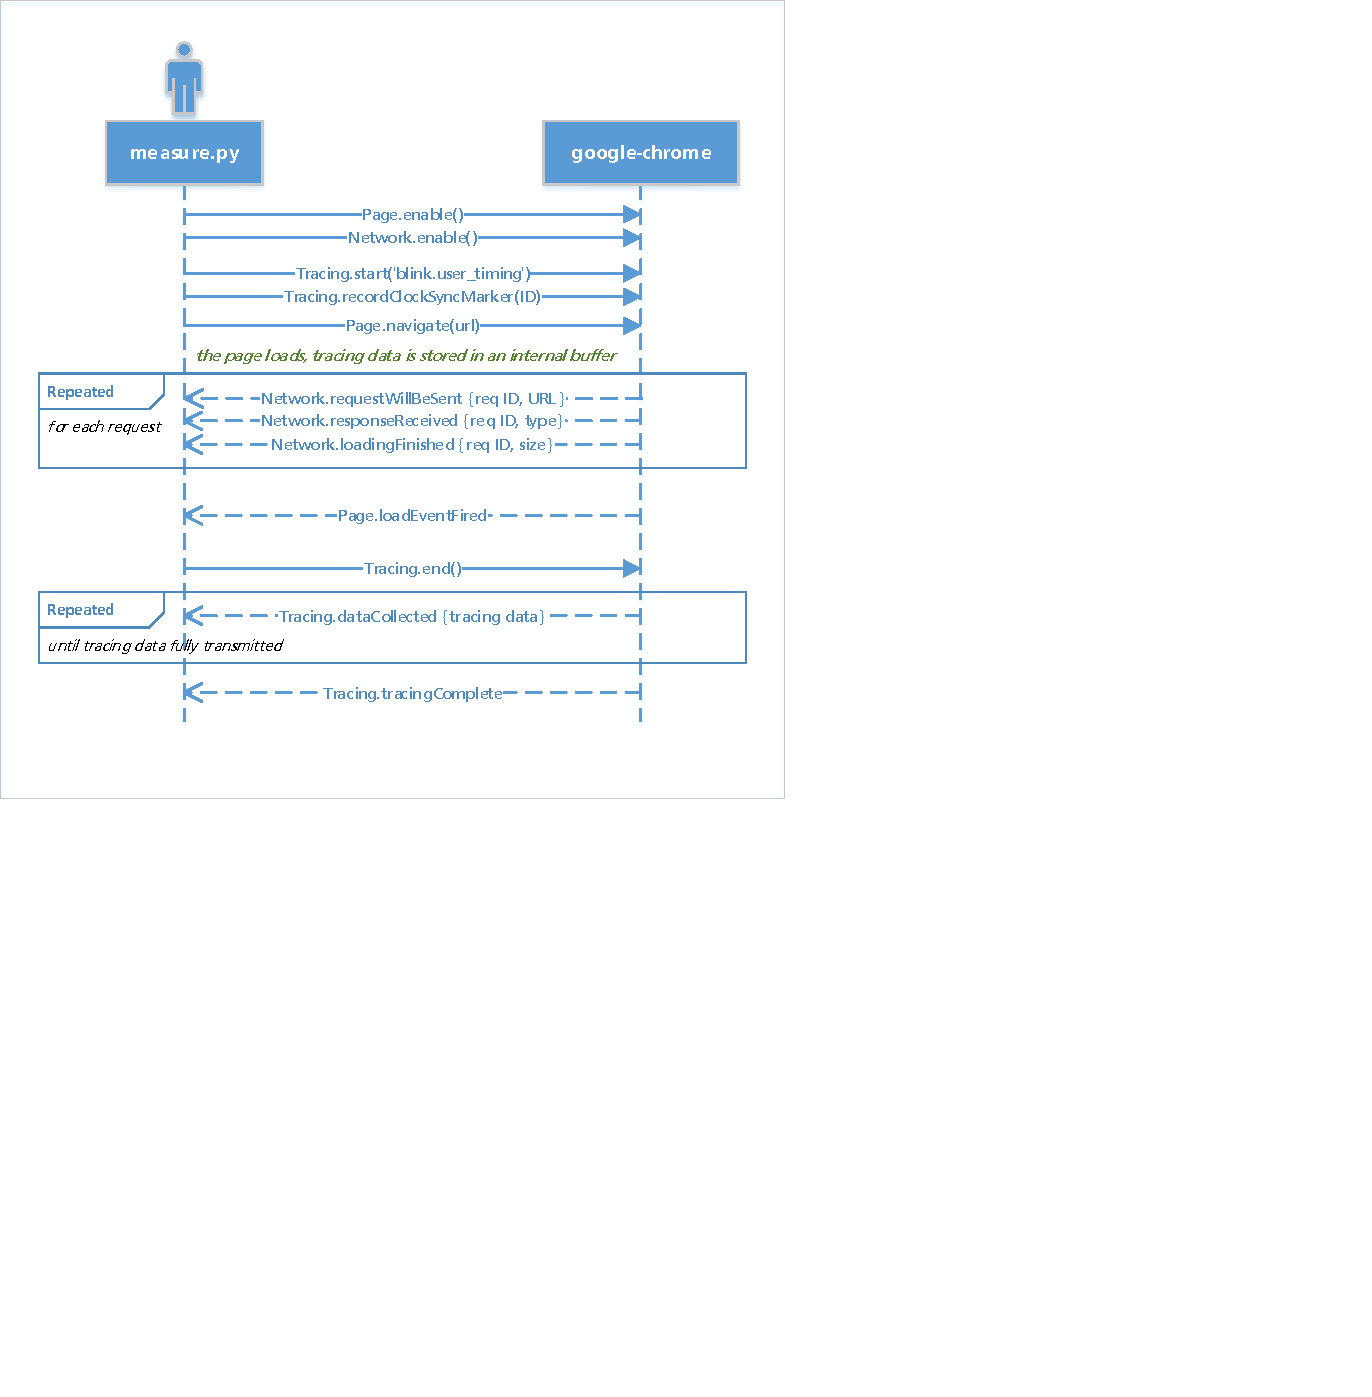
\includegraphics[width=0.45\textwidth, trim=0.25in 0.25in 0.25in 0.25in, clip]{chrome-tracing.pdf}
	\caption{A sample interaction with the Chrome Tracing API}
	\label{fig:chrome-tracing-api}
\end{wrapfigure}


When evaluating the performance of web page loads, there are several metrics to look at. We use three timing metrics, which are available over the Chrome debugging protocol\footnote{\url{https://developer.chrome.com/devtools/docs/debugger-protocol}}, the protocol of the Google Chrome web browser's developer tools.

%Parameters/Properties/Values: (in order of usual occurence)


% DOMContentLoaded
The \textit{DOMContentLoaded} event is fired after the main HTML document has been fully received and parsed by the browser. As the parsing is blocked by synchronous JavaScript, this event can't be fired before scripts have been downloaded and executed. Style sheets do not block parsing, but are recommended to be referenced before JavaScript files, so they will usually be loaded as well.

The browser can start rendering the page before the DOM is fully loaded, but only does this if loading the DOM takes exceptionally long (multiple seconds). 
%browsers can render before domcontentloaded, but are very relucant to do so. only if loading the document itself takes several seconds, they start rendering. they display a white screen or the web page that was open before 


% First Meaningful Paint
The \textit{First Contentful Paint} is the time when the first text, image or similar object is painted on screen. On most pages, the first object is a header or navigation bar \cite{Sakamoto2016TTFMP}, making this metric less useful for the purpose of measuring the time until useful content for the user is visible. We use the \textit{First Meaningful Paint} metric instead, which \textcite{Sakamoto2016TTFMP} defines as ``the time when page's primary content appeared on the screen.'' They emphasize that ``[d]efinitions of primary content differ depending on pages. For blog articles, it would be the headline + above-the-fold text (and text must be visible -- not waiting for fonts). For search engines, it would be search results. If an image is critical to the page (e.g. e-commerce product page), then first meaningful paint requires it to be visible.'' Therefore, to measure the first meaningful paint accurately, it would be necessary for the user to define the primary content. In the developer tools of Google Chrome, it is implemented using a heuristics based on the number of layout objects, page height and web font loading.



% Page Load Time (i.e. time until the onLoad event)
The third metric we measure is the \textit{Page Load Time}, i.e. the time of the \textit{load} event. This is the time it takes to load all embedded resources, like style sheets, web fonts and images. 

A Python script is used to instrument the browser to load pages, and to record the times at which the events noted above occur over the Chrome debugging protocol. A sample interaction with the browser over the API is shown in Figure \ref{fig:chrome-tracing-api}.


\section{Measurement Environments}

We based our measurements on two different methods. We simulated network situations with Mininet, which constructs a completely virtual environment on a single computer. This approach has the benefit of being fairly reproducible, because no-one else uses the virtual network and causes uncontrollable variations. On the other hand, the simulation only represents part of the reality, therefore we also conducted evaluations on real networks. This trades reproducibility for a more realistic environment, including congestion on intermediate routers, packet loss on Wi-Fi and cellular links, and other behaviour of real networks, which is quite complex.


\subsection{Mininet}

\todo{short intro to mininet}

\todo{our setup with mininet}

\todo{...}



\subsubsection{TCP Small Queues}

If there is a stall below the TCP layer, the TCP small queues \cite{LwnTSQ} algorithm ensures not too much data gets buffered in the fifos of network interfaces, e.g. when an applications send data faster than the network interface card can relay it. To do this, the algorithm checks \code{sk_wmem_alloc}, a field of the socket struct in the kernel, which stores the amount of memory currently used for the send buffer. The default multipath scheduler in the Linux kernel declares a subflow as temporarily unavailable if the underlying TCP socket is throttled, as seen in Listing \ref{lst:mptcp_is_temp_unavailable}. When using RBS, the information if a subflow is throttled is available as the property \code{<subflow>.THROTTLED} and can be considered in the scheduling decision.

\begin{lstlisting}[label=lst:mptcp_is_temp_unavailable,caption={Excerpt from Multipath TCP Kernel, \code{net/mptcp/mptcp_sched.c}
%\footnote{url{https://github.com/multipath-tcp/mptcp/blob/e076f6be0f4b3d48d59c686d0a9ff4b87bc91a0f/net/mptcp/mptcp\_sched.c\#L39}}
}]
static bool mptcp_is_temp_unavailable(struct sock *sk,
				      const struct sk_buff *skb,
				      bool zero_wnd_test)
{
 [...]
	/* If TSQ is already throttling us, do not send on this subflow. When
	 * TSQ gets cleared the subflow becomes eligible again.
	 */
	if (test_bit(TSQ_THROTTLED, &tp->tsq_flags))
		return true;
\end{lstlisting}

This is where a difference between simulated and real networks exists: in Mininet the TCP Small Queue throttling never got engaged, because \code{sk_wmem_alloc} never changes from its initial value of \code{1}. This is consequential, as the virtual ethernet devices don't have to really transmit any data, instead only passing along a pointer, and therefore never need to buffer it.

In our simulations, each packet is delayed in the network emulation (netem) layer, and traffic shaping is used, to simulate a real link with latency and limited bandwidth. This layer resides between the TCP stack and the virtual ethernet device, therefore it should cause \code{sk_wmem_alloc} to increase, but it didn't.
%-        Gilt das auch f�r shaping ohne delay, e.g., 10 Mbit bw? W�rde es ohne den patch also mit 10Mbit und ohne delay �wie erwartet� laufen?
When using only traffic shaping, but not the delaying functionality of netem, the problem does not occur. 

%https://kernelnewbies.org/Linux_3.6#head-b1e33c4c78affb4186e5affc4b4a2bc7d44a3e66
%https://lwn.net/Articles/507065/

So we built a test case where a delay is added on one host with netem\footnote{\code{tc qdisc add dev h1-eth0 root netem delay 5000ms}}, and then \code{iperf} is run to create traffic between the host. We also added a debug output to the function \code{tcp_small_queue_check} in \code{net/ipv4/tcp_output.c} \footnote{\url{http://lxr.free-electrons.com/source/net/ipv4/tcp_output.c\#L2074}} to see if TSQ will throttle the output. But in Mininet / veth, \code{sk_wmem_alloc} is always at the value \code{1}. The \code{TSQ_THROTTLED} never gets set. If doing the same on two machines connected over ethernet cable, \code{sk_wmem_alloc} raises, and eventually \code{TSQ_THROTTLED} is set.

An inquiry on the Mininet mailing list resulted\footnote{\url{https://mailman.stanford.edu/pipermail/mininet-discuss/2017-April/007425.html}} in the hint that the latency emulation code calls \code{skb_orphan_partial}, which reduces the socket buffer's size to \code{1}, therefore essentially removing it from \code{sk_wmem_alloc}.
This further lead us to a code comment in the Linux kernel which says that this behaviour is by design, because ``orphaning usually takes place at TX completion time, so \_before\_ the link transit delay'' (Linux kernel 4.4, \code{net/sched/sch_netem.c}, line 429). 
%-        Netem delay packets werden EXTRA rausgenommen, weil?
The reason is that the netem layer is designed to emulate delays in the \textit{network}, not \textit{network interface}, to test e.g. TCP congestion control algorithms. Therefore it needs to behave as if the delay occured after orphaning the socket buffer.  But we want do emulate delays in the \textit{network interface} in this case, so we change this behaviour by commenting out the call to \code{skb_orphan_partial} as shown in Listing \ref{lst:sch_netem}. To see if the call would have been normally made, we also added a debug output temporarily. This enabled us to test the TSQ throttling in our simulation with Mininet.


\begin{lstlisting}[label=lst:sch_netem,caption={Modified version of Linux kernel 4.4, \code{net/sched/sch_netem.c}}]
398 /*
399  * Insert one skb into qdisc.
400  * Note: parent depends on return value to account for queue length.
401  *      NET_XMIT_DROP: queue length didn't change.
402  *      NET_XMIT_SUCCESS: one skb was queued.
403  */
404 static int netem_enqueue(struct sk_buff *skb, struct Qdisc *sch)
405 {
 [...]
429         /* If a delay is expected, orphan the skb. (orphaning usually takes
430          * place at TX completion time, so _before_ the link transit delay)
431          */
432         // if (q->latency || q->jitter)
433         //         skb_orphan_partial(skb);
434
435         printk("netem_enqueue: ...not calling skb_orphan_partial latency=%ld, jitter=%ld, sk=%p, sk_wmem_alloc=%d", 
436                q->latency, q->jitter, skb->sk, skb->sk == NULL ? 0 : atomic_read(&skb->sk->sk_wmem_alloc));
\end{lstlisting}








\subsection{Real World Measurements}

To confirm the measurements we conducted in Mininet, we ran the same software on real hardware and real networks. For the server side, we used a virtual machine located in the Frankfurt data center of Amazon Web Services and another one in the Roubaix data center of OVH. As clients, we used notebooks connected to the internet via Wi-Fi and DSL, via a Wi-Fi hotspot with VPN tunneling, and via USB to a mobile phone with an LTE connection.\footnote{We were unable to use the university's internet connection directly as its Firewall blocks Multipath TCP connections.}

\todo{more details about the measurement setup?}



\section{Evaluations}

\todo{something}

\subsection{Evaluation A}
% zeigen - implementiertung funktioniert grunds�tzlich
% simple (``academic'') content-type specific scheduling

The goal of this evaluation is to test the implementation of content-type specific scheduling, and to show a first content-type based optimization of a synthetic web page. The network situation is shown in Figure \ref{eva1-scenario}. A user with a smart phone is connected to a free Wi-Fi hotspot, which routes the traffic through a VPN and therefore incurs a high latency, and is also connected to a cellular network with low latency but metered traffic limits. The user loads a web page which is modelled after a typical news article, it consists of an HTML document referencing style sheet, script and images of different size. All styles and scripts are included in the \code{<head>} of the document and required for rendering the page. Two big images are included below the fold and are not required for the rendering.

The scenario is emulated in Mininet. Client and Server are modelled as Mininet hosts running the Google Chrome browser and the nghttpd web server, respectively. They each have two interfaces, which are connected by two Mininet links with delay and rate limiting to simulate the two connection paths. 

A scheduler script was designed to send the images only over the ``cheap'' Wi-Fi subflow, and allow the other, more time-critical data, to choose from the available subflows the one with the lowest round-trip time.

\begin{lstlisting}
/*
 * This scheduler sends packets on the subflow with the lowest RTT which has congestion window available
 *  ... except images, they are sent only on the "cheap" (non-backup) subflow (e.g. Wi-Fi instead of 3G)
*/
SCHEDULER min_rtt_ctype_aware;

VAR SKB_CONTENT_NOSTREAM = 1;
VAR SKB_CONTENT_DOCUMENT = 2;
VAR SKB_CONTENT_SCRIPT   = 3;
VAR SKB_CONTENT_STYLE    = 4;
VAR SKB_CONTENT_IMAGE    = 5;
VAR SKB_CONTENT_OTHER    = 6;

/* only use subflows which have CWND left*/
VAR usableSbfs = SUBFLOWS.FILTER(sbf => sbf.CWND > sbf.SKBS_IN_FLIGHT);

/* no subflows available? do nothing. */
IF (usableSbfs.EMPTY) { RETURN; }

/* send packets from resend buffer redundantly on the fastest new subflows */
IF (!RQ.EMPTY) {
	usableSbfs.FILTER(sbf => !RQ.TOP.SENT_ON(sbf)).MIN(sbf => sbf.RTT).PUSH(RQ.POP());
	RETURN;
}

IF (!Q.EMPTY) {
	/* simplified content type is passed along by the web server */
	VAR content_type = Q.TOP.USER;

	IF (Q.TOP.USER >= SKB_CONTENT_IMAGE) {
		/* the subflows marked as "BACKUP" are filtered out */
		usableSbfs.FILTER(sbf => !sbf.IS_BACKUP).MIN(sbf => sbf.RTT).PUSH(Q.POP());
	} ELSE {
		usableSbfs.MIN(sbf => sbf.RTT).PUSH(Q.POP());
	}
}
\end{lstlisting}


\begin{figure}
\centering
	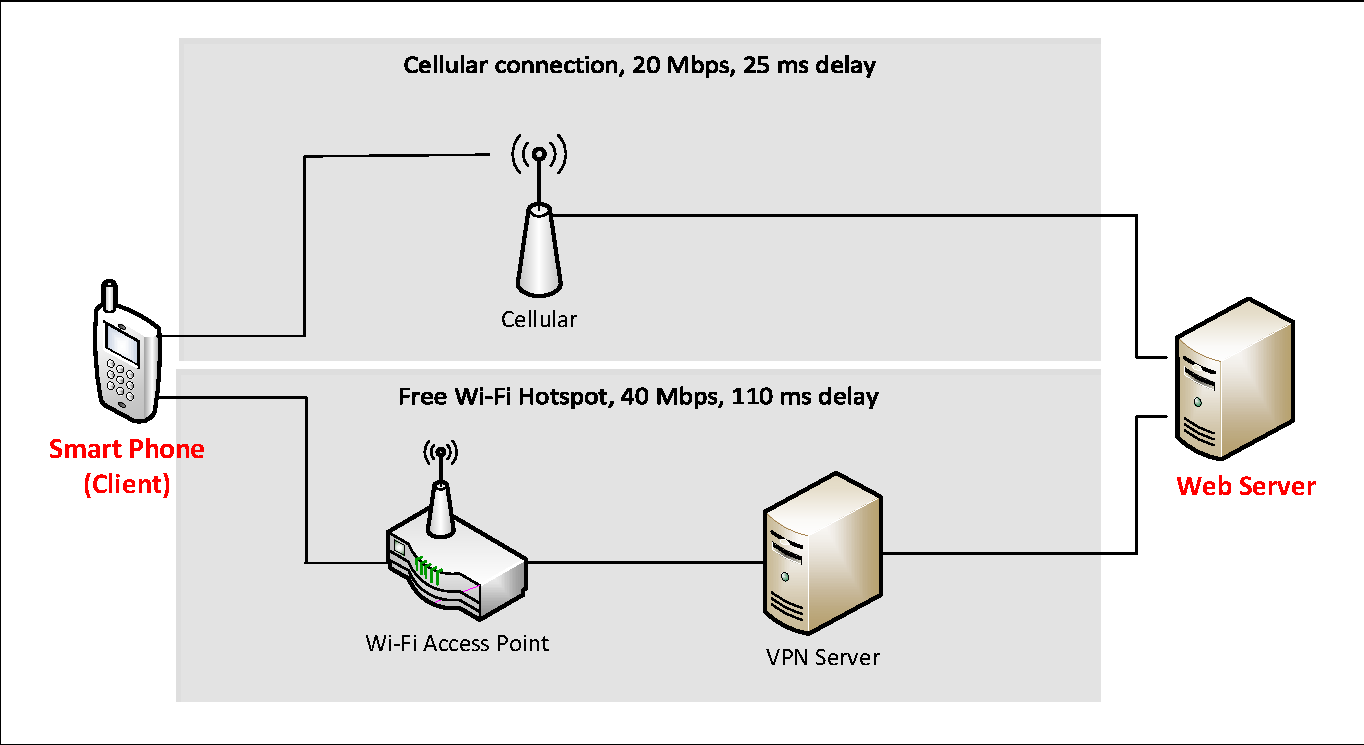
\includegraphics[width=0.9\textwidth]{eva1-scenario.pdf}
	\caption{Network scenario which is simulated in Evaluation A }
	\label{eva1-scenario}
\end{figure}

\begin{figure}
\centering
	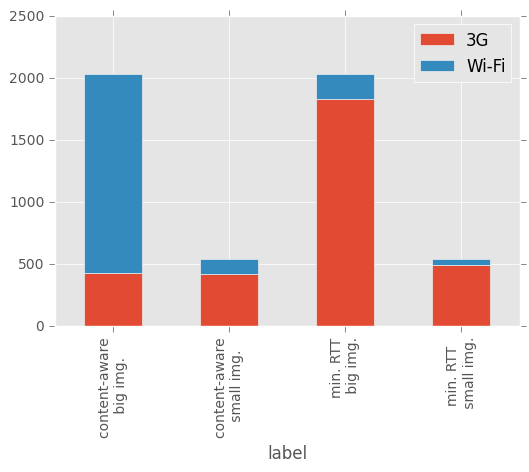
\includegraphics[width=0.45\textwidth]{eva1-rxbytes.png}
	\caption{Received bytes per interface for Evaluation A }
	\label{eva1-rxbytes}
\end{figure}

\begin{figure}
\centering
	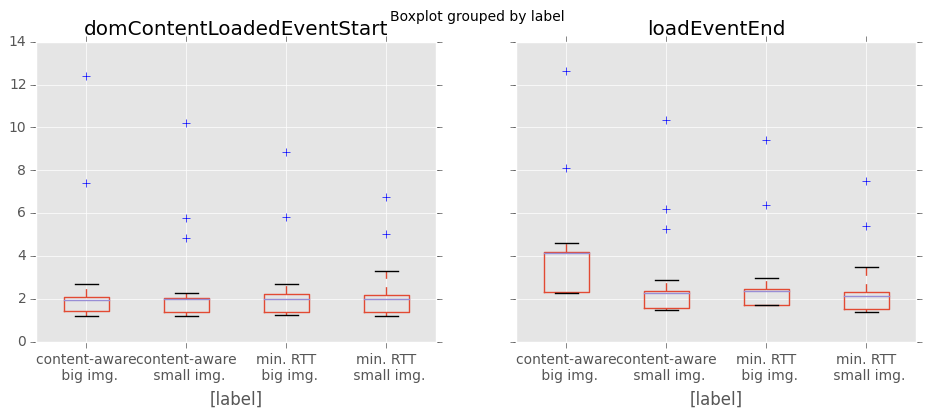
\includegraphics[width=0.9\textwidth]{eva1-loadtimes.png}
	\caption{Page load times for Evaluation A }
	\label{eva1-loadtimes}
\end{figure}


% simulated netw. with mininet
% - two hosts, two paths
% - path one (slow Wi-Fi hotspot, e.g. over vpn) - bw=50, delay=110
% - path two (LTE) - bw=50, delay=50
% server: nghttpd, modified for RBS socket options
% - hint: content type (document, style, script, image, other)
% scheduler: rbs
% - forTest: script 1: redundant for document+style
% - forTest: script 2: never transmit images on LTE
% baselines:
% - script 3: redundant scheduler (everything redundant)
% - linux mptcp default scheduler
% - single path tcp on Wi-Fi
% - single path tcp on LTE
% web site:
% - synthetic web site with:




% later ajax redundant
% oder images only one sbf












%=====================================================================
\chapter{Conclusion}
%=====================================================================



\section{Outlook / Future Work}

The client (web browser) side of optimizations was mostly excluded from our considerations. 
% one might implement a mptcp protocol extension so the logic can sit mostly in browser OR webserver, and the other side is instructed what to do
% another way to generalize this could be definining a way for the web page/app to give the hints to the browser, which passes them on to the client mptcp scheduler
% -> the server scheduler implementation could send the corresponding mptcp frames with the same scheduling strategy as the request

% on the other hand, a different, quite simple approach could be taken on the browser side: send regular GET requests (maybe also POST with small body) as fast, latency critical strategy, while sending big POSTs (uploads) as latency uncritical strategy
% it might be possible to do a good heuristical approach here, without support from the browser, only in the mptcp scheduler



% Extension to three or more interfaces


% our work could be combined with :
Some optimizations rely on manually providing resource priorities and dependencies to the web server. Our work could be combined with automated algorithms to determine dependency graphs of web pages and user relevancy ratings of resources. Butkiewicz et al. \cite{klotski2015}

% - automated categorization of ressources/http requests

% - automated dependency graph

%Automatische Einstufung von Seitenbestandteilen (HTTP Requests) in Relevanz / User Utility
%-> nicht Thema der Arbeit, aber evtl. relevant f�r praktische Umsetzung

%Automatisches Aufbauen von Dependency Graphs



%=====================================================================
% Bibliography
%=====================================================================


\nocite{*}
%\chapter{Bibliography}
%\bibliography{thesis-h2-mptcp}{}
\printbibliography




\end{document}
